\documentclass[12pt]{article}
\usepackage{amsmath,amssymb,amsfonts}
\usepackage{graphicx}
\usepackage{algorithm}
\usepackage{algpseudocode}
\usepackage{enumitem}
\usepackage[margin=1in]{geometry}
\usepackage{xcolor}
\usepackage{tcolorbox}
\usepackage{tikz}
\usepackage{hyperref}
\tcbuselibrary{theorems, breakable} % <-- add breakable here

\hypersetup{
    colorlinks=true,
    linkcolor=blue,
    filecolor=magenta,
    urlcolor=cyan,
}

\tcbuselibrary{theorems}

\newtcbtheorem[number within=section]{example}{Example}{
  colback=green!5,
  colframe=green!35!black,
  fonttitle=\bfseries,
  enhanced,
  breakable, % <-- add this line
  attach boxed title to top left={yshift=-2mm, xshift=2mm},
  boxed title style={colback=green!35!black}
}{ex}

\newtcbtheorem[number within=section]{definition}{Definition}{
  colback=blue!5,
  colframe=blue!35!black,
  fonttitle=\bfseries,
  enhanced,
  breakable, % <-- add this line
  attach boxed title to top left={yshift=-2mm, xshift=2mm},
  boxed title style={colback=blue!35!black}
}{def}

\newtcbtheorem[number within=section]{algorithmenv}{Algorithm}{
  colback=red!5,
  colframe=red!35!black,
  fonttitle=\bfseries,
  enhanced,
  breakable, % <-- add this line
  attach boxed title to top left={yshift=-2mm, xshift=2mm},
  boxed title style={colback=red!35!black}
}{alg}

\begin{document}

\title{Mathematical Foundations of Machine Learning\\Comprehensive Study Guide}
\author{For Students}
\date{\today}
\maketitle

\tableofcontents
\newpage

\section{Exam Structure and Preparation Strategy}

\begin{tcolorbox}[title=Exam Format, colback=yellow!5, colframe=yellow!50!black]
\begin{itemize}
    \item \textbf{Concepts and Definitions:} 10 questions, 5 points each (50 points total)
    \item \textbf{Mathematical Derivations/Solutions:} 3 problems, 25 points each (75 points total)
    \item Maximum possible score: 100 points
\end{itemize}
\end{tcolorbox}

\begin{tcolorbox}[title=Study Strategy, colback=yellow!5, colframe=yellow!50!black]
\begin{enumerate}
    \item \textbf{Understand core concepts first} - Focus on intuition before diving into mathematics
    \item \textbf{Practice derivations} - Work through examples step-by-step
    \item \textbf{Connect theory to applications} - Relate concepts to engineering problems
    \item \textbf{Visualize algorithms} - Draw flowcharts or diagrams to understand processes
    \item \textbf{Implement simple examples} - Code basic versions of algorithms if time permits
\end{enumerate}
\end{tcolorbox}

\section{Core Concepts and Definitions}

\subsection{Supervised Machine Learning} %% ====================================

\begin{definition}{Supervised Learning}{supervised-learning}
A type of machine learning where an algorithm learns a function $f: \mathcal{X} \rightarrow \mathcal{Y}$ from labeled training data consisting of input-output pairs $(x_i, y_i)$. The goal is to predict outputs for new, unseen inputs.
\end{definition}

\begin{example}{Supervised Learning in Engineering}{supervised-engineering}
\textbf{Structural Engineering Application:} Predicting building stress under different loads.

\begin{itemize}
    \item \textbf{Inputs $\mathcal{X}$:} Building dimensions, material properties, load configurations
    \item \textbf{Outputs $\mathcal{Y}$:} Maximum stress values at critical points
    \item \textbf{Training data:} Historical measurements or finite element simulations
    \item \textbf{Model:} Could be linear regression for simple cases or neural networks for complex geometries
\end{itemize}

The trained model allows quick stress estimation without running expensive simulations for each new design.
\end{example}

\begin{algorithmenv}{Supervised Learning Process}{supervised-algorithm}
\begin{algorithmic}[1]
\State \textbf{Input:} Training data $\{(x_1, y_1), (x_2, y_2), \ldots, (x_n, y_n)\}$
\State \textbf{Output:} A function $f$ that maps inputs to outputs
\State Choose a model class (e.g., linear, tree-based, neural network)
\State Define a loss function $L(y, f(x))$ to measure prediction error
\State Initialize model parameters $\theta$
\While{not converged}
    \State Compute predictions $\hat{y}_i = f_\theta(x_i)$ for all training examples
    \State Compute loss $J(\theta) = \frac{1}{n}\sum_{i=1}^n L(y_i, \hat{y}_i)$
    \State Update parameters $\theta$ to reduce loss (e.g., using gradient descent)
\EndWhile
\State \textbf{return} trained model $f_\theta$
\end{algorithmic}
\end{algorithmenv}


\subsection{Overfitting}

\begin{definition}{Overfitting}{overfitting}
Overfitting occurs when a model learns the training data too well, capturing noise rather than the underlying pattern. This results in poor generalization to new, unseen data.
\end{definition}

\begin{example}{Overfitting in Signal Processing}{overfitting-engineering}
\textbf{Sensor Calibration Problem:} An engineer needs to calibrate a temperature sensor based on 10 measurements.

\begin{itemize}
    \item \textbf{Simple model (linear):} $T = 0.95V + 2.3$ has 5°C average error
    \item \textbf{Complex model (high-degree polynomial):} Passes through all 10 points exactly (0°C training error)
\end{itemize}

When tested on new measurements, the linear model maintains ~5°C error, but the polynomial model shows large errors. The polynomial captured measurement noise rather than the true relationship.

\begin{center}
\begin{tikzpicture}[scale=0.6]
\draw[->] (0,0) -- (10,0) node[right] {Voltage};
\draw[->] (0,0) -- (0,8) node[above] {Temperature};
\foreach \x/\y in {1/1.2, 2/2.3, 3/3.1, 4/3.8, 5/5.2, 6/5.7, 7/6.9, 8/7.3, 9/8.1, 10/9.2}
    \fill (\x,\y) circle (3pt);
\draw[thick, blue] (0,2.3) -- (10,11.8) node[right] {Linear model};
% Simplified illustrative curve instead of complex polynomial
\draw[thick, red, domain=1:10, samples=50, smooth] plot (\x, {0.05*(\x-5)^3 + 0.2*(\x-5)^2 + 0.5*(\x-5) + 5}) node[right] {Overfitted model};
\end{tikzpicture}
\end{center}
\end{example}




\subsection{Multi-class Classification with Binary Classifiers}

\begin{definition}{Multi-class Classification}{multiclass}
The task of classifying instances into one of three or more classes. When using binary classifiers (which distinguish between only two classes), special strategies are needed.
\end{definition}

\begin{example}{Multi-class Classification in Fault Diagnosis}{multiclass-engineering}
\textbf{Motor Fault Detection:} An engineer needs to classify motor faults into 4 categories: bearing failure, stator winding fault, rotor bar damage, and normal operation.

\textbf{One-vs-Rest (OvR) approach:}
\begin{itemize}
    \item Train 4 binary classifiers:
    \begin{itemize}
        \item Classifier 1: Bearing failure vs. Others
        \item Classifier 2: Stator winding fault vs. Others
        \item Classifier 3: Rotor bar damage vs. Others
        \item Classifier 4: Normal operation vs. Others
    \end{itemize}
    \item For a new vibration signal, run all 4 classifiers
    \item Assign the class with highest confidence score
\end{itemize}

\textbf{One-vs-One (OvO) approach:}
\begin{itemize}
    \item Train 6 binary classifiers (one for each pair of classes)
    \item For a new signal, get votes from all classifiers
    \item Assign the class with most votes
\end{itemize}

\begin{center}
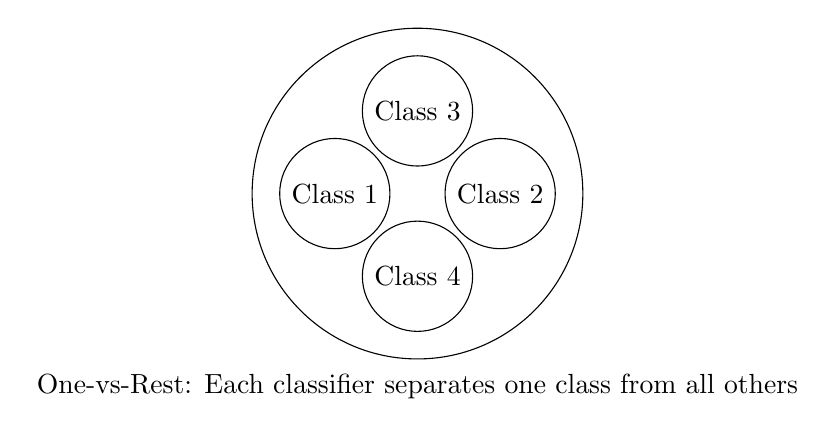
\begin{tikzpicture}[scale=0.7]
\draw (0,0) circle (3cm);
\draw (-1.5,0) circle (1cm);
\draw (1.5,0) circle (1cm);
\draw (0,1.5) circle (1cm);
\draw (0,-1.5) circle (1cm);
\node at (-1.5,0) {Class 1};
\node at (1.5,0) {Class 2};
\node at (0,1.5) {Class 3};
\node at (0,-1.5) {Class 4};
\node at (0,-3.5) {One-vs-Rest: Each classifier separates one class from all others};
\end{tikzpicture}
\end{center}
\end{example}

\begin{algorithmenv}{One-vs-Rest (OvR) Implementation}{ovr-algorithm}
\begin{algorithmic}[1]
\State \textbf{Input:} Training data $\{(x_i, y_i)\}$ where $y_i \in \{1,2,\ldots,K\}$
\State \textbf{Output:} Set of $K$ binary classifiers
\For{$k = 1$ to $K$}
    \State Create binary labels: $z_i = 1$ if $y_i = k$, else $z_i = 0$
    \State Train binary classifier $f_k$ on $\{(x_i, z_i)\}$
\EndFor
\State \textbf{Prediction for new input $x$:}
\State Compute scores $s_k = f_k(x)$ for all $k$
\State Return $\arg\max_k s_k$ as predicted class
\end{algorithmic}
\end{algorithmenv}

\subsection{Stochastic Gradient Descent}

\begin{definition}{Stochastic Gradient Descent (SGD)}{sgd}
An optimization algorithm that updates model parameters using gradients computed from a single randomly selected training example (or mini-batch) at each iteration, rather than the entire dataset.
\end{definition}

\begin{example}{SGD in Adaptive Control Systems}{sgd-engineering}
\textbf{Adaptive Filter Design:} An engineer is designing a noise cancellation system that must adapt to changing environments.

\textbf{Problem:} Minimize error in the filter output by adjusting filter coefficients.

\textbf{Traditional approach:} Collect 1000 samples, compute optimal coefficients, then apply.
\begin{itemize}
    \item \textbf{Issue:} Environment changes before computation completes
\end{itemize}

\textbf{SGD approach:} Update filter coefficients after each new sample.
\begin{itemize}
    \item \textbf{Benefit:} Filter adapts in real-time to changing conditions
    \item \textbf{Implementation:} $w_{t+1} = w_t - \eta \nabla E_t(w_t)$ where $E_t$ is error for sample $t$
\end{itemize}

\begin{center}
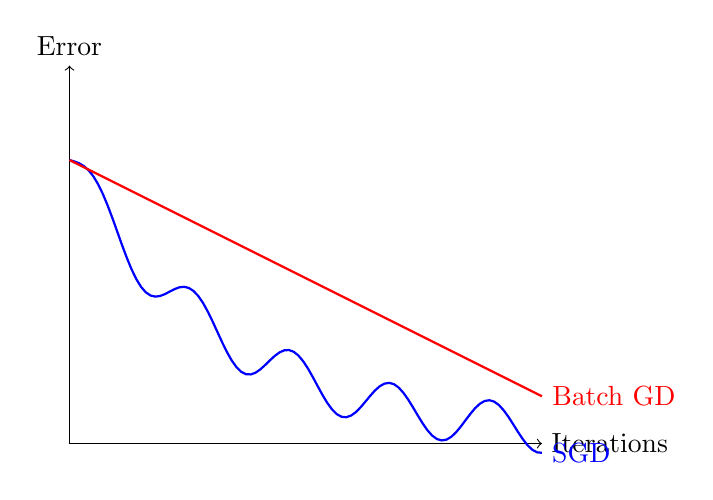
\begin{tikzpicture}[scale=0.6]
\draw[->] (0,0) -- (10,0) node[right] {Iterations};
\draw[->] (0,0) -- (0,8) node[above] {Error};
\draw[thick, blue, domain=0:10, samples=100] plot (\x, {6*exp(-0.3*\x) + 0.5*sin(3*\x r)}) node[right] {SGD};
\draw[thick, red] (0,6) -- (10,1) node[right] {Batch GD};
\end{tikzpicture}
\end{center}
\end{example}

\begin{algorithmenv}{Stochastic Gradient Descent}{sgd-algorithm}
\begin{algorithmic}[1]
\State \textbf{Input:} Training data $\{(x_i, y_i)\}$, learning rate $\eta$, iterations $T$
\State \textbf{Output:} Optimized parameters $\theta$
\State Initialize parameters $\theta_0$
\For{$t = 1$ to $T$}
    \State Randomly select training example $(x_i, y_i)$
    \State Compute gradient $g_t = \nabla_\theta L(\theta_{t-1}, x_i, y_i)$
    \State Update parameters: $\theta_t = \theta_{t-1} - \eta g_t$
\EndFor
\State \textbf{return} $\theta_T$
\end{algorithmic}
\end{algorithmenv}



\subsection{BFGS Algorithm}

\begin{definition}{BFGS Algorithm}{bfgs}
A quasi-Newton optimization method that approximates the inverse Hessian matrix to achieve faster convergence than first-order methods like gradient descent, without explicitly computing second derivatives.
\end{definition}

\begin{example}{BFGS in Structural Optimization}{bfgs-engineering}
\textbf{Truss Design Optimization:} An engineer needs to find the optimal cross-sectional areas for members in a truss to minimize weight while meeting stress constraints.

\textbf{Problem characteristics:}
\begin{itemize}
    \item 50 design variables (member areas)
    \item Nonlinear stress constraints
    \item Objective function is weight (linear)
    \item Gradient can be computed analytically
    \item Hessian would be expensive to compute
\end{itemize}

\textbf{BFGS approach:}
\begin{itemize}
    \item Start with identity matrix as initial Hessian approximation
    \item Update approximation based on gradient changes
    \item Converges in 28 iterations vs. 120+ for gradient descent
\end{itemize}

\begin{center}
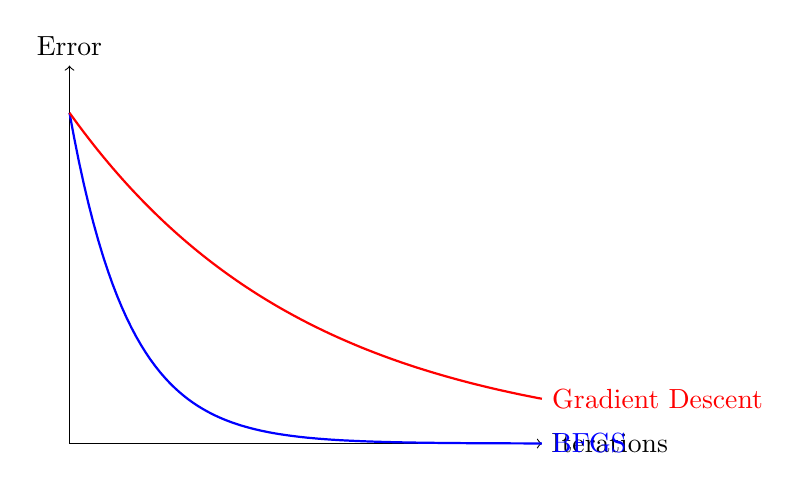
\begin{tikzpicture}[scale=0.6]
\draw[->] (0,0) -- (10,0) node[right] {Iterations};
\draw[->] (0,0) -- (0,8) node[above] {Error};
\draw[thick, blue, domain=0:10, samples=100] plot (\x, {7*exp(-0.8*\x)}) node[right] {BFGS};
\draw[thick, red, domain=0:10, samples=100] plot (\x, {7*exp(-0.2*\x)}) node[right] {Gradient Descent};
\end{tikzpicture}
\end{center}
\end{example}

\begin{algorithmenv}{BFGS Algorithm}{bfgs-algorithm}
\begin{algorithmic}[1]
\State \textbf{Input:} Function $f$, gradient $\nabla f$, initial point $x_0$, convergence tolerance $\epsilon$
\State \textbf{Output:} Local minimum $x^*$
\State Initialize $k = 0$, $B_0 = I$ (identity matrix)
\While{$\|\nabla f(x_k)\| > \epsilon$}
    \State Compute search direction $d_k = -B_k \nabla f(x_k)$
    \State Find step size $\alpha_k$ using line search
    \State Update: $x_{k+1} = x_k + \alpha_k d_k$
    \State Define $s_k = x_{k+1} - x_k$ and $y_k = \nabla f(x_{k+1}) - \nabla f(x_k)$
    \State Update inverse Hessian approximation:
    \State $B_{k+1} = (I - \frac{s_k y_k^T}{y_k^T s_k})B_k(I - \frac{y_k s_k^T}{y_k^T s_k}) + \frac{s_k s_k^T}{y_k^T s_k}$
    \State $k = k + 1$
\EndWhile
\State \textbf{return} $x_k$
\end{algorithmic}
\end{algorithmenv}

\subsection{Logistic Regression as a Probabilistic Model}

\begin{definition}{Logistic Regression}{logistic-regression}
A statistical model that uses the logistic function to model a binary dependent variable. It directly estimates the probability of an event occurring, making it inherently probabilistic.
\end{definition}

\begin{example}{Logistic Regression in Reliability Engineering}{logistic-engineering}
\textbf{Component Failure Prediction:} An engineer wants to predict the probability of electronic component failure based on operating temperature and voltage.

\textbf{Data:} 200 components tested under various conditions, with binary outcome (failed/not failed).

\textbf{Logistic model:}
\begin{align}
P(\text{failure}) &= \frac{1}{1 + e^{-(b_0 + b_1 \cdot \text{temp} + b_2 \cdot \text{voltage})}} \\
\log\left(\frac{P(\text{failure})}{1-P(\text{failure})}\right) &= b_0 + b_1 \cdot \text{temp} + b_2 \cdot \text{voltage}
\end{align}

\textbf{Fitted model:} $\log\left(\frac{P(\text{failure})}{1-P(\text{failure})}\right) = -12.3 + 0.15 \cdot \text{temp} + 0.08 \cdot \text{voltage}$

\textbf{Interpretation:} 
\begin{itemize}
    \item For each 1°C increase in temperature, the odds of failure increase by a factor of $e^{0.15} = 1.16$ (16\%)
    \item For a component operating at 80°C and 5V, the failure probability is:
    \begin{align}
    P(\text{failure}) &= \frac{1}{1 + e^{-((-12.3) + 0.15 \cdot 80 + 0.08 \cdot 5)}} \\
    &= \frac{1}{1 + e^{-((-12.3) + 12 + 0.4)}} \\
    &= \frac{1}{1 + e^{-0.1}} \\
    &\approx 0.525 \text{ or } 52.5\%
    \end{align}
\end{itemize}

\begin{center}
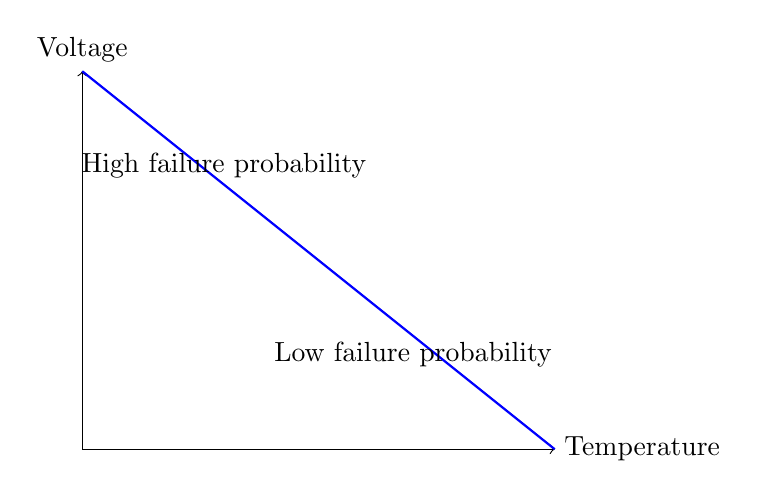
\begin{tikzpicture}[scale=0.6]
\draw[->] (0,0) -- (10,0) node[right] {Temperature};
\draw[->] (0,0) -- (0,8) node[above] {Voltage};
\draw[thick, blue] (0,8) -- (10,0);
\node at (3,6) {High failure probability};
\node at (7,2) {Low failure probability};
\end{tikzpicture}
\end{center}
\end{example}

\begin{algorithmenv}{Logistic Regression Training}{logistic-algorithm}
\begin{algorithmic}[1]
\State \textbf{Input:} Training data $\{(x_i, y_i)\}$ where $y_i \in \{0,1\}$
\State \textbf{Output:} Parameters $\theta = [w, b]$
\State Initialize $\theta_0$
\State Define sigmoid function $\sigma(z) = \frac{1}{1+e^{-z}}$
\State Define loss function $J(\theta) = -\frac{1}{n}\sum_{i=1}^n [y_i \log(\sigma(w^T x_i + b)) + (1-y_i)\log(1-\sigma(w^T x_i + b))]$
\While{not converged}
    \State Compute predictions $\hat{y}_i = \sigma(w^T x_i + b)$
    \State Update $w = w - \alpha \frac{1}{n}\sum_{i=1}^n (\hat{y}_i - y_i)x_i$
    \State Update $b = b - \alpha \frac{1}{n}\sum_{i=1}^n (\hat{y}_i - y_i)$
\EndWhile
\State \textbf{return} $\theta = [w, b]$
\end{algorithmic}
\end{algorithmenv}

\subsection{Support Vector Machine}

\begin{definition}{Support Vector Machine (SVM)}{svm}
A supervised learning model that finds the optimal hyperplane that maximizes the margin between classes, where the margin is defined as the distance between the hyperplane and the nearest data point from either class.
\end{definition}

\begin{example}{SVM in Materials Science}{svm-engineering}
\textbf{Material Classification:} An engineer needs to classify materials as ductile or brittle based on composition percentages of two alloying elements.

\textbf{Data:} 50 samples with known classifications and measured properties.

\textbf{SVM approach:}
\begin{itemize}
    \item Find the widest possible "street" (margin) between ductile and brittle materials
    \item The boundary of this street is defined by the support vectors
    \item New materials are classified based on which side of the street they fall on
\end{itemize}

\textbf{Mathematical formulation:}
\begin{align}
\min_{w,b} &\frac{1}{2}\|w\|^2 \\
\text{subject to } &y_i(w^T x_i + b) \geq 1 \text{ for all } i
\end{align}

\begin{center}
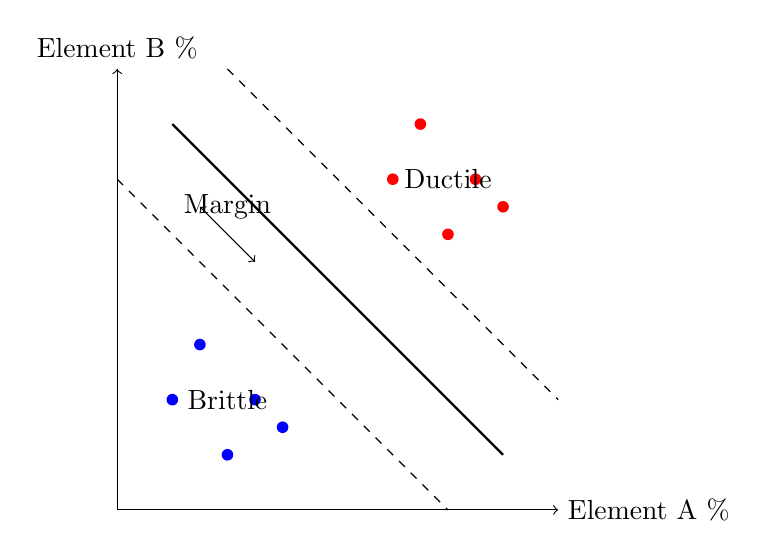
\begin{tikzpicture}[scale=0.7]
\draw[->] (0,0) -- (8,0) node[right] {Element A \%};
\draw[->] (0,0) -- (0,8) node[above] {Element B \%};
\draw[thick] (1,7) -- (7,1);
\draw[dashed] (2,8) -- (8,2);
\draw[dashed] (0,6) -- (6,0);
\foreach \x/\y in {1/2, 2/1, 1.5/3, 2.5/2, 3/1.5}
    \fill[blue] (\x,\y) circle (3pt);
\foreach \x/\y in {5/6, 6/5, 5.5/7, 6.5/6, 7/5.5}
    \fill[red] (\x,\y) circle (3pt);
\draw[<->] (1.5,5.5) -- (2.5,4.5);
\node at (2,5.5) {Margin};
\node at (2,2) {Brittle};
\node at (6,6) {Ductile};
\end{tikzpicture}
\end{center}
\end{example}

\begin{algorithmenv}{Support Vector Machine Training}{svm-algorithm}
\begin{algorithmic}[1]
\State \textbf{Input:} Training data $\{(x_i, y_i)\}$ where $y_i \in \{-1,1\}$
\State \textbf{Output:} Parameters $w, b$ defining the hyperplane
\State Formulate the dual problem:
\State $\max_\alpha \sum_{i=1}^n \alpha_i - \frac{1}{2}\sum_{i=1}^n\sum_{j=1}^n \alpha_i \alpha_j y_i y_j x_i^T x_j$
\State subject to $\alpha_i \geq 0$ and $\sum_{i=1}^n \alpha_i y_i = 0$
\State Solve for $\alpha$ using quadratic programming
\State Compute $w = \sum_{i=1}^n \alpha_i y_i x_i$
\State Find $b$ using support vectors (points where $\alpha_i > 0$):
\State $b = \frac{1}{N_{sv}} \sum_{i \in SV} (y_i - w^T x_i)$
\State \textbf{return} $w, b$
\end{algorithmic}
\end{algorithmenv}



\subsection{The Kernel Trick}

\begin{definition}{Kernel Trick}{kernel-trick}
A mathematical technique that allows algorithms to operate in a high-dimensional feature space without explicitly computing coordinates in that space, by expressing operations solely in terms of inner products in the original space.
\end{definition}

\begin{example}{Kernel Trick in Signal Processing}{kernel-engineering}
\textbf{Nonlinear Signal Classification:} An engineer needs to classify signals as either normal or faulty based on frequency characteristics that are not linearly separable.

\textbf{Original features:} Two frequency components $x = [f_1, f_2]$

\textbf{Without kernel trick:}
\begin{itemize}
    \item Explicitly map to higher dimensions: $\phi(x) = [f_1, f_2, f_1^2, f_2^2, f_1f_2]$
    \item Compute SVM in 5-dimensional space (computationally expensive)
\end{itemize}

\textbf{With kernel trick:}
\begin{itemize}
    \item Define polynomial kernel: $K(x, z) = (x^T z + 1)^2$
    \item For $x = [f_1, f_2]$ and $z = [z_1, z_2]$:
    \begin{align}
    K(x, z) &= (f_1z_1 + f_2z_2 + 1)^2 \\
    &= f_1^2z_1^2 + f_2^2z_2^2 + 2f_1f_2z_1z_2 + 2f_1z_1 + 2f_2z_2 + 1 \\
    &= \phi(x)^T\phi(z)
    \end{align}
    \item Compute SVM using only kernel function (much more efficient)
\end{itemize}

\begin{center}
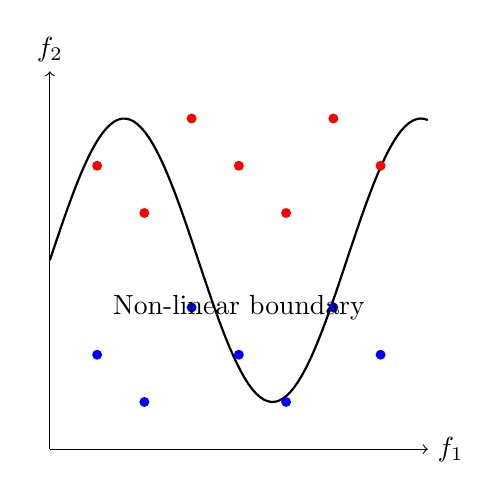
\begin{tikzpicture}[scale=0.6]
\draw[->] (0,0) -- (8,0) node[right] {$f_1$};
\draw[->] (0,0) -- (0,8) node[above] {$f_2$};
\draw[thick, domain=0:8, samples=100] plot (\x, {4 + 3*sin(\x r)});
\foreach \x/\y in {1/2, 2/1, 3/3, 4/2, 5/1, 6/3, 7/2}
    \fill[blue] (\x,\y) circle (3pt);
\foreach \x/\y in {1/6, 2/5, 3/7, 4/6, 5/5, 6/7, 7/6}
    \fill[red] (\x,\y) circle (3pt);
\node at (4,3) {Non-linear boundary};
\end{tikzpicture}
\end{center}
\end{example}

\begin{algorithmenv}{Kernel SVM Algorithm}{kernel-svm-algorithm}
\begin{algorithmic}[1]
\State \textbf{Input:} Training data $\{(x_i, y_i)\}$, kernel function $K$
\State \textbf{Output:} Parameters $\alpha, b$ for decision function
\State Formulate the dual problem with kernel:
\State $\max_\alpha \sum_{i=1}^n \alpha_i - \frac{1}{2}\sum_{i=1}^n\sum_{j=1}^n \alpha_i \alpha_j y_i y_j K(x_i, x_j)$
\State subject to $\alpha_i \geq 0$ and $\sum_{i=1}^n \alpha_i y_i = 0$
\State Solve for $\alpha$ using quadratic programming
\State Find $b$ using support vectors:
\State $b = \frac{1}{N_{sv}} \sum_{i \in SV} (y_i - \sum_{j \in SV} \alpha_j y_j K(x_j, x_i))$
\State \textbf{Decision function:} $f(x) = \text{sign}(\sum_{i \in SV} \alpha_i y_i K(x_i, x) + b)$
\State \textbf{return} $\alpha, b$
\end{algorithmic}
\end{algorithmenv}

\subsection{KKT Conditions}

\begin{definition}{Karush-Kuhn-Tucker (KKT) Conditions}{kkt}
Necessary conditions for a solution to be optimal in constrained optimization problems. They extend the method of Lagrange multipliers to inequality constraints.
\end{definition}

\begin{example}{KKT Conditions in Resource Allocation}{kkt-engineering}
\textbf{Power Distribution Problem:} An engineer must allocate power to 3 subsystems to maximize performance while meeting constraints.

\textbf{Optimization problem:}
\begin{align}

%%====================================================================

\max_{P_1, P_2, P_3} f(P_1, P_2, P_3) = 2\ln(P_1) + 3\ln(P_2) + \ln(P_3)
\end{align}

\textbf{Subject to constraints:}
\begin{align}
P_1 + P_2 + P_3 &\leq 100 \text{ (total power constraint)} \\
P_1 &\geq 10 \text{ (minimum power for subsystem 1)} \\
P_2 &\geq 15 \text{ (minimum power for subsystem 2)} \\
P_3 &\geq 5 \text{ (minimum power for subsystem 3)}
\end{align}

\textbf{KKT approach:}
\begin{enumerate}
    \item \textbf{Form the Lagrangian:}
    \begin{align}
    \mathcal{L} = 2\ln(P_1) + 3\ln(P_2) + \ln(P_3) - \lambda_1(P_1 + P_2 + P_3 - 100) \\
    + \lambda_2(P_1 - 10) + \lambda_3(P_2 - 15) + \lambda_4(P_3 - 5)
    \end{align}
    
    \item \textbf{KKT conditions:}
    \begin{align}
    \frac{\partial \mathcal{L}}{\partial P_1} &= \frac{2}{P_1} - \lambda_1 + \lambda_2 = 0 \\
    \frac{\partial \mathcal{L}}{\partial P_2} &= \frac{3}{P_2} - \lambda_1 + \lambda_3 = 0 \\
    \frac{\partial \mathcal{L}}{\partial P_3} &= \frac{1}{P_3} - \lambda_1 + \lambda_4 = 0 \\
    \lambda_1(P_1 + P_2 + P_3 - 100) &= 0 \text{ (complementary slackness)} \\
    \lambda_2(P_1 - 10) &= 0 \text{ (complementary slackness)} \\
    \lambda_3(P_2 - 15) &= 0 \text{ (complementary slackness)} \\
    \lambda_4(P_3 - 5) &= 0 \text{ (complementary slackness)} \\
    P_1 + P_2 + P_3 &\leq 100, P_1 \geq 10, P_2 \geq 15, P_3 \geq 5 \text{ (primal feasibility)} \\
    \lambda_1, \lambda_2, \lambda_3, \lambda_4 &\geq 0 \text{ (dual feasibility)}
    \end{align}
\end{enumerate}

\textbf{Solution:} From the nature of the objective function (increasing with power), we know the total power constraint will be tight: $P_1 + P_2 + P_3 = 100$ and $\lambda_1 > 0$.

From the first three equations and assuming no minimum constraints are binding:
\begin{align}
P_1 &= \frac{2}{\lambda_1} \\
P_2 &= \frac{3}{\lambda_1} \\
P_3 &= \frac{1}{\lambda_1}
\end{align}

Substituting into the power constraint:
\begin{align}
\frac{2}{\lambda_1} + \frac{3}{\lambda_1} + \frac{1}{\lambda_1} &= 100 \\
\frac{6}{\lambda_1} &= 100 \\
\lambda_1 &= \frac{6}{100} = 0.06
\end{align}

Therefore:
\begin{align}
P_1 &= \frac{2}{0.06} = 33.33 \\
P_2 &= \frac{3}{0.06} = 50 \\
P_3 &= \frac{1}{0.06} = 16.67
\end{align}

Since all minimum constraints are satisfied, this is our optimal solution.
\end{example}

\begin{algorithmenv}{Solving Optimization Problems with KKT Conditions}{kkt-algorithm}
\begin{algorithmic}[1]
\State \textbf{Input:} Objective function $f(x)$, equality constraints $h_i(x) = 0$, inequality constraints $g_j(x) \leq 0$
\State \textbf{Output:} Optimal solution $x^*$
\State Form the Lagrangian: $\mathcal{L}(x, \lambda, \mu) = f(x) - \sum_i \lambda_i h_i(x) - \sum_j \mu_j g_j(x)$
\State Write out the KKT conditions:
\State \quad Stationarity: $\nabla_x \mathcal{L}(x, \lambda, \mu) = 0$
\State \quad Primal feasibility: $h_i(x) = 0$ and $g_j(x) \leq 0$
\State \quad Dual feasibility: $\mu_j \geq 0$
\State \quad Complementary slackness: $\mu_j g_j(x) = 0$
\State Solve the system of equations and inequalities
\State Verify second-order conditions if necessary
\State \textbf{return} $x^*$
\end{algorithmic}
\end{algorithmenv}

\subsection{Mini-batch Learning}

\begin{definition}{Mini-batch Learning}{mini-batch}
A training technique that uses small random subsets (mini-batches) of the training data for each parameter update, combining aspects of both stochastic and batch gradient descent.
\end{definition}

\begin{example}{Mini-batch Learning in Autonomous Vehicle Training}{mini-batch-engineering}
\textbf{Obstacle Detection System:} An engineer is training a neural network to detect obstacles from camera images for an autonomous vehicle.

\textbf{Dataset:} 100,000 labeled images (obstacle/no obstacle)

\textbf{Training approaches comparison:}
\begin{itemize}
    \item \textbf{Batch gradient descent:} Use all 100,000 images for each parameter update
    \begin{itemize}
        \item Pros: Stable convergence, accurate gradient
        \item Cons: Requires 50GB of memory, each epoch takes 30 minutes
    \end{itemize}
    
    \item \textbf{Stochastic gradient descent:} Use 1 random image for each update
    \begin{itemize}
        \item Pros: Low memory requirement, frequent updates
        \item Cons: Extremely noisy updates, poor convergence
    \end{itemize}
    
    \item \textbf{Mini-batch learning (batch size = 64):} Use 64 random images for each update
    \begin{itemize}
        \item Pros: Reasonable memory requirement (200MB), good parallelization on GPU
        \item Cons: Still some noise in updates, requires tuning batch size
    \end{itemize}
\end{itemize}

\textbf{Results:} Mini-batch approach reaches 95\% accuracy in 2 hours, compared to 5 hours for batch gradient descent and 3 hours for SGD (but with lower 92\% accuracy).
\end{example}

\begin{algorithmenv}{Mini-batch Gradient Descent}{mini-batch-algorithm}
\begin{algorithmic}[1]
\State \textbf{Input:} Training data $\{(x_i, y_i)\}_{i=1}^n$, batch size $b$, learning rate $\alpha$, epochs $E$
\State \textbf{Output:} Optimized parameters $\theta$
\State Initialize parameters $\theta_0$
\For{$e = 1$ to $E$}
    \State Shuffle training data
    \For{$t = 1$ to $\lceil n/b \rceil$}
        \State Select mini-batch: $\mathcal{B}_t = \{(x_i, y_i)\}_{i=(t-1)b+1}^{\min(tb, n)}$
        \State Compute gradient on mini-batch: $g_t = \frac{1}{|\mathcal{B}_t|} \sum_{(x,y) \in \mathcal{B}_t} \nabla_\theta \mathcal{L}(f_\theta(x), y)$
        \State Update parameters: $\theta_t = \theta_{t-1} - \alpha \cdot g_t$
    \EndFor
\EndFor
\State \textbf{return} $\theta$
\end{algorithmic}
\end{algorithmenv}

\subsection{Curse of Dimensionality}

\begin{definition}{Curse of Dimensionality}{curse-dimensionality}
A phenomenon where the amount of data needed to make statistically sound predictions grows exponentially with the dimensionality of the feature space, making analysis increasingly difficult in high-dimensional spaces.
\end{definition}

\begin{example}{Curse of Dimensionality in Structural Health Monitoring}{curse-engineering}
\textbf{Bridge Monitoring System:} An engineer is developing a system to detect structural damage using sensor data.

\textbf{Data collection:}
\begin{itemize}
    \item 50 sensors on the bridge, each collecting 10 features (frequency response, temperature effects, etc.)
    \item Total: 500-dimensional feature vector for each measurement
\end{itemize}

\textbf{Problems encountered:}
\begin{itemize}
    \item To adequately cover the 500D space, exponentially more data points are needed
    \item With only 1,000 measurements, the space is extremely sparse
    \item Distance metrics become less meaningful (most points are approximately equidistant)
    \item Model requires 100,000+ parameters, risking severe overfitting
\end{itemize}

\textbf{Solutions applied:}
\begin{itemize}
    \item \textbf{Feature selection:} Engineering knowledge to select 20 most relevant features
    \item \textbf{Principal Component Analysis:} Reduced 500D to 15D while preserving 95\% of variance
    \item \textbf{Autoencoder:} Neural network to learn a 10D representation of the data
\end{itemize}

\textbf{Results:} Damage detection accuracy improved from 65\% to 92\% after dimensionality reduction.

\begin{center}
\begin{tikzpicture}[scale=0.7]
\draw[->] (0,0) -- (8,0) node[right] {Number of dimensions};
\draw[->] (0,0) -- (0,6) node[above] {Data points needed};
\draw[thick, domain=1:7, samples=100] plot (\x, {0.1*2^(\x)});
\node at (4,4) {Exponential growth};
\end{tikzpicture}
\end{center}
\end{example}

\begin{algorithmenv}{Dimensionality Reduction with PCA}{pca-algorithm}
\begin{algorithmic}[1]
\State \textbf{Input:} Data matrix $X \in \mathbb{R}^{n \times d}$, target dimensionality $k$
\State \textbf{Output:} Reduced data $Z \in \mathbb{R}^{n \times k}$
\State Center the data: $X_c = X - \mu_X$ where $\mu_X$ is the mean of each feature
\State Compute covariance matrix: $\Sigma = \frac{1}{n}X_c^T X_c$
\State Find eigenvalues and eigenvectors of $\Sigma$
\State Sort eigenvectors by decreasing eigenvalues
\State Select top $k$ eigenvectors to form projection matrix $W \in \mathbb{R}^{d \times k}$
\State Project data: $Z = X_c W$
\State \textbf{return} $Z$
\end{algorithmic}
\end{algorithmenv}


\subsection{Gaussian Homotopy Continuation}

\begin{definition}{Gaussian Homotopy Continuation}{homotopy}
A numerical method for solving systems of nonlinear equations by gradually transforming a simple problem with known solution into the target problem, using a continuous deformation parameter.
\end{definition}

\begin{example}{Homotopy in Circuit Design Optimization}{homotopy-engineering}
\textbf{Nonlinear Circuit Optimization:} An electrical engineer needs to find optimal component values for a circuit with highly nonlinear behavior.

\textbf{Problem:} Find values for resistors $R_1, R_2$ and capacitor $C$ that satisfy a system of nonlinear equations:
\begin{align}
f_1(R_1, R_2, C) &= 0 \\
f_2(R_1, R_2, C) &= 0 \\
f_3(R_1, R_2, C) &= 0
\end{align}

\textbf{Direct approach:} Newton's method fails due to poor initial guess.

\textbf{Homotopy approach:}
\begin{enumerate}
    \item Start with simplified circuit model with known solution $(R_1^0, R_2^0, C^0)$
    \item Define homotopy function: $H(R_1, R_2, C, t) = (1-t)G(R_1, R_2, C) + tF(R_1, R_2, C)$
    where $G$ is the simplified model and $F$ is the target model
    \item Gradually increase $t$ from 0 to 1, tracking the solution path
    \item At each step, use previous solution as starting point for next step
\end{enumerate}

\textbf{Results:} Successfully found solution $(R_1^*, R_2^*, C^*)$ that standard optimization methods missed.

\begin{center}
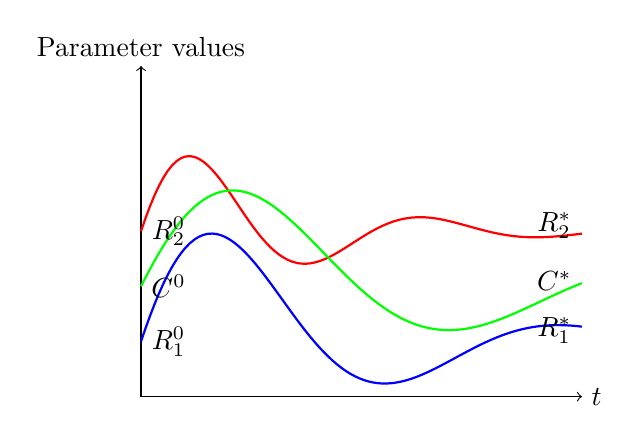
\begin{tikzpicture}[scale=0.7]
\draw[->] (0,0) -- (8,0) node[right] {$t$};
\draw[->] (0,0) -- (0,6) node[above] {Parameter values};
\draw[thick, blue, domain=0:8, samples=100] plot (\x, {1 + 3*exp(-0.3*\x)*sin(\x r)});
\draw[thick, red, domain=0:8, samples=100] plot (\x, {3 + 2*exp(-0.4*\x)*sin(1.5*\x r)});
\draw[thick, green, domain=0:8, samples=100] plot (\x, {2 + 2.5*exp(-0.2*\x)*sin(0.8*\x r)});
\node at (0.5,1) {$R_1^0$};
\node at (7.5,1.2) {$R_1^*$};
\node at (0.5,3) {$R_2^0$};
\node at (7.5,3.1) {$R_2^*$};
\node at (0.5,2) {$C^0$};
\node at (7.5,2.1) {$C^*$};
\end{tikzpicture}
\end{center}
\end{example}

\begin{algorithmenv}{Gaussian Homotopy Continuation Method}{homotopy-algorithm}
\begin{algorithmic}[1]
\State \textbf{Input:} Target system $F(x) = 0$, start system $G(x) = 0$ with known solution $x_0$, steps $N$
\State \textbf{Output:} Solution to target system $x^*$
\State Define homotopy $H(x, t) = (1-t)G(x) + tF(x)$
\State Initialize $x = x_0$ and $t = 0$
\For{$i = 1$ to $N$}
    \State $t_i = i/N$
    \State Predictor step: Estimate $\tilde{x}_i$ using tangent to solution path at $(x_{i-1}, t_{i-1})$
    \State Corrector step: Refine $x_i$ by solving $H(x, t_i) = 0$ starting from $\tilde{x}_i$
\EndFor
\State \textbf{return} $x_N$ as approximation to $x^*$
\end{algorithmic}
\end{algorithmenv}

\subsection{Decision Tree Classifier Objective}

\begin{definition}{Decision Tree Objective}{decision-tree}
The goal of a decision tree classifier is to create a model that recursively partitions the feature space to maximize the homogeneity (or minimize the impurity) of the target variable within each partition.
\end{definition}

\begin{example}{Decision Tree in Manufacturing Quality Control}{decision-tree-engineering}
\textbf{Product Defect Classification:} A manufacturing engineer needs to identify causes of product defects.

\textbf{Data:} 1,000 products with 5 features (temperature, pressure, material batch, operator ID, machine ID) and binary outcome (defective/non-defective).

\textbf{Decision tree approach:}
\begin{itemize}
    \item Start with all 1,000 products (15\% defective)
    \item Find best feature to split on: Temperature (< 150°C vs. ≥ 150°C)
    \item Left branch: 600 products (5\% defective)
    \item Right branch: 400 products (30\% defective)
    \item Continue splitting right branch by Pressure
    \item Continue until stopping criteria met
\end{itemize}

\textbf{Objective function:} Information Gain = Parent Entropy - Weighted Sum of Child Entropy

For temperature split:
\begin{align}
\text{Parent entropy} &= -0.15\log_2(0.15) - 0.85\log_2(0.85) = 0.61 \\
\text{Left entropy} &= -0.05\log_2(0.05) - 0.95\log_2(0.95) = 0.29 \\
\text{Right entropy} &= -0.30\log_2(0.30) - 0.70\log_2(0.70) = 0.88 \\
\text{Information gain} &= 0.61 - (0.6 \cdot 0.29 + 0.4 \cdot 0.88) = 0.61 - 0.53 = 0.08
\end{align}

\begin{center}
\begin{tikzpicture}[scale=0.7, level distance=1.5cm, sibling distance=3cm]
\node {All: 15\% defective}
    child {node {Temp < 150°C\\5\% defective}}
    child {node {Temp ≥ 150°C\\30\% defective}
        child {node {Pressure < 50 bar\\10\% defective}}
        child {node {Pressure ≥ 50 bar\\45\% defective}}
    };
\end{tikzpicture}
\end{center}
\end{example}

\begin{algorithmenv}{Decision Tree Training Algorithm}{decision-tree-algorithm}
\begin{algorithmic}[1]
\State \textbf{Input:} Training data $\{(x_i, y_i)\}$, maximum depth $d_{max}$, minimum samples per leaf $n_{min}$
\State \textbf{Output:} Decision tree model
\Function{BuildTree}{data, depth}
    \If{stopping criteria met (depth = $d_{max}$ or samples ≤ $n_{min}$ or pure node)}
        \State \Return leaf node with majority class
    \EndIf
    \State Find best feature $j$ and threshold $t$ that maximizes information gain
    \State Split data into left ($x_j < t$) and right ($x_j \geq t$) subsets
    \State left\_subtree = BuildTree(left\_subset, depth+1)
    \State right\_subtree = BuildTree(right\_subset, depth+1)
    \State \Return decision node with feature $j$, threshold $t$, left and right subtrees
\EndFunction
\State \textbf{return} BuildTree(training\_data, 0)
\end{algorithmic}
\end{algorithmenv}

\subsection{k-Nearest Neighbors Classifier}

\begin{definition}{k-Nearest Neighbors (k-NN)}{knn}
A non-parametric classification method that assigns a class to a new data point based on the majority class among its $k$ nearest neighbors in the training set, where "nearest" is defined by a distance metric.
\end{definition}

\begin{example}{k-NN in Materials Science}{knn-engineering}
\textbf{Alloy Property Prediction:} A materials engineer needs to predict the yield strength of a new alloy based on its composition.

\textbf{Data:} 200 alloys with known compositions (percentages of 5 elements) and measured yield strengths.

\textbf{k-NN approach:}
\begin{itemize}
    \item For a new alloy with composition [0.7, 0.1, 0.05, 0.1, 0.05]
    \item Compute Euclidean distance to all 200 known alloys
    \item Select $k=5$ nearest neighbors
    \item Predict yield strength as average of these 5 neighbors
\end{itemize}

\textbf{Distance calculation example:}
\begin{align}
d(\text{new}, \text{alloy}_i) &= \sqrt{\sum_{j=1}^5 (x_{\text{new},j} - x_{i,j})^2} \\
&= \sqrt{(0.7-0.65)^2 + (0.1-0.15)^2 + \ldots} \\
&= 0.08
\end{align}

\textbf{Results:} The 5 nearest neighbors have yield strengths [350, 370, 345, 360, 355] MPa, so the predicted yield strength is 356 MPa.

\begin{center}
\begin{tikzpicture}[scale=0.7]
\draw[->] (0,0) -- (8,0) node[right] {Element A \%};
\draw[->] (0,0) -- (0,8) node[above] {Element B \%};
\foreach \x/\y/\s in {1/2/320, 2/1/290, 3/3/330, 4/2/310, 5/6/380, 6/5/370, 5.5/7/390, 6.5/6/385, 7/5.5/375, 2/6/350, 3/5/345, 2.5/5.5/355, 3.5/4.5/340, 4.5/3.5/335}
    \fill[blue] (\x,\y) circle (3pt) node[font=\tiny] {\s};
\fill[red] (3,4) circle (5pt) node[font=\tiny, above] {?};
\draw[dashed] (3,4) circle (1.5cm);
\end{tikzpicture}
\end{center}
\end{example}

\begin{algorithmenv}{k-Nearest Neighbors Algorithm}{knn-algorithm}
\begin{algorithmic}[1]
\State \textbf{Input:} Training data $\{(x_i, y_i)\}$, new point $x_{new}$, number of neighbors $k$, distance metric $d$
\State \textbf{Output:} Predicted class $\hat{y}_{new}$
\For{$i = 1$ to $n$}
    \State Compute distance $d_i = d(x_i, x_{new})$
\EndFor
\State Find indices $\{i_1, i_2, \ldots, i_k\}$ of the $k$ smallest distances
\State For classification: $\hat{y}_{new} = \text{majority class among } \{y_{i_1}, y_{i_2}, \ldots, y_{i_k}\}$
\State For regression: $\hat{y}_{new} = \frac{1}{k}\sum_{j=1}^k y_{i_j}$
\State \textbf{return} $\hat{y}_{new}$
\end{algorithmic}
\end{algorithmenv}

\subsection{Complementary Slackness}

\begin{definition}{Complementary Slackness}{complementary-slackness}
A condition in constrained optimization stating that for each inequality constraint, either the constraint is active (equality holds) or its corresponding Lagrange multiplier is zero.
\end{definition}

\begin{example}{Complementary Slackness in Resource Allocation}{complementary-engineering}
\textbf{Manufacturing Optimization:} An engineer must allocate machine time to maximize profit while respecting constraints.

\textbf{Problem:}
\begin{align}
\max_{x_1, x_2} &\; 5x_1 + 3x_2 \text{ (profit)} \\
\text{subject to: } &x_1 + x_2 \leq 10 \text{ (total machine hours)} \\
&x_1 \leq 7 \text{ (material 1 availability)} \\
&x_2 \leq 5 \text{ (material 2 availability)} \\
&x_1, x_2 \geq 0 \text{ (non-negativity)}
\end{align}

\textbf{Lagrangian:}
\begin{align}
\mathcal{L} = 5x_1 + 3x_2 - \lambda_1(x_1 + x_2 - 10) - \lambda_2(x_1 - 7) - \lambda_3(x_2 - 5)
\end{align}

\textbf{KKT conditions:}
\begin{align}
\frac{\partial \mathcal{L}}{\partial x_1} &= 5 - \lambda_1 - \lambda_2 = 0 \\
\frac{\partial \mathcal{L}}{\partial x_2} &= 3 - \lambda_1 - \lambda_3 = 0
\end{align}

\textbf{Complementary slackness:}
\begin{align}
\lambda_1(x_1 + x_2 - 10) &= 0 \\
\lambda_2(x_1 - 7) &= 0 \\
\lambda_3(x_2 - 5) &= 0
\end{align}

\textbf{Solution:} Since profit is maximized by producing as much as possible, and product 1 is more profitable, we expect $x_1 = 7$ (material 1 constraint binding) and $x_2 = 3$ to use all 10 machine hours.

Checking complementary slackness:
\begin{itemize}
    \item $\lambda_1 > 0$ because total machine hours constraint is binding
    \item $\lambda_2 > 0$ because material 1 constraint is binding
    \item $\lambda_3 = 0$ because material 2 constraint is not binding
\end{itemize}

From the gradient conditions:
\begin{align}
5 - \lambda_1 - \lambda_2 &= 0 \\
3 - \lambda_1 - 0 &= 0 \Rightarrow \lambda_1 = 3
\end{align}

Therefore $\lambda_2 = 5 - 3 = 2$, confirming our analysis.
\end{example}

\begin{algorithmenv}{Checking Complementary Slackness}{complementary-algorithm}
\begin{algorithmic}[1]
\State \textbf{Input:} Solution $x^*$, Lagrange multipliers $\lambda^*$, constraints $g_i(x) \leq 0$
\State \textbf{Output:} Whether complementary slackness is satisfied
\For{each constraint $i$}
    \State Check if $\lambda_i^* \cdot g_i(x^*) = 0$
    \If{$\lambda_i^* > 0$ and $g_i(x^*) < 0$}
        \State \textbf{return} False (complementary slackness violated)
    \EndIf
    \If{$\lambda_i^* = 0$ and $g_i(x^*) = 0$}
        \State This is a degenerate case (constraint active but multiplier zero)
    \EndIf
\EndFor
\State \textbf{return} True (complementary slackness satisfied)
\end{algorithmic}
\end{algorithmenv}




\section{Mathematical Derivations and Solutions}

\subsection{Problem 1: Training a Simple Classifier}

\begin{example}{Logistic Regression Training Iteration}{logistic-training}
\textbf{Problem:} Train a logistic regression model on the following small dataset for 2 iterations:

\begin{center}
\begin{tabular}{|c|c|c|c|}
\hline
Example & $x_1$ & $x_2$ & $y$ \\
\hline
1 & 2 & 1 & 1 \\
2 & 1 & 3 & 1 \\
3 & 0 & 0 & 0 \\
4 & 1 & 1 & 0 \\
\hline
\end{tabular}
\end{center}

Starting with $w_1 = 0$, $w_2 = 0$, $b = 0$, and learning rate $\eta = 0.1$.

\textbf{Solution approach:}

1. \textbf{Logistic function:} $\sigma(z) = \frac{1}{1+e^{-z}}$ where $z = w_1x_1 + w_2x_2 + b$

2. \textbf{Prediction:} $\hat{y} = \sigma(z)$

3. \textbf{Cost function:} $J(w,b) = -\frac{1}{m}\sum_{i=1}^{m}[y_i\log(\hat{y}_i) + (1-y_i)\log(1-\hat{y}_i)]$

4. \textbf{Gradient:}
   \begin{align}
   \frac{\partial J}{\partial w_j} &= \frac{1}{m}\sum_{i=1}^{m}(\hat{y}_i - y_i)x_{ij} \\
   \frac{\partial J}{\partial b} &= \frac{1}{m}\sum_{i=1}^{m}(\hat{y}_i - y_i)
   \end{align}

5. \textbf{Update rule:}
   \begin{align}
   

   %% =================================================================================

      w_j &= w_j - \eta \frac{\partial J}{\partial w_j} \\
   b &= b - \eta \frac{\partial J}{\partial b}
   \end{align}

\textbf{Iteration 1:}

\textbf{Initial parameters:} $w_1 = 0$, $w_2 = 0$, $b = 0$

\textbf{For each example:}
\begin{itemize}
    \item Example 1: $z = 0 \cdot 2 + 0 \cdot 1 + 0 = 0$, $\hat{y}_1 = \sigma(0) = 0.5$
    \item Example 2: $z = 0 \cdot 1 + 0 \cdot 3 + 0 = 0$, $\hat{y}_2 = \sigma(0) = 0.5$
    \item Example 3: $z = 0 \cdot 0 + 0 \cdot 0 + 0 = 0$, $\hat{y}_3 = \sigma(0) = 0.5$
    \item Example 4: $z = 0 \cdot 1 + 0 \cdot 1 + 0 = 0$, $\hat{y}_4 = \sigma(0) = 0.5$
\end{itemize}

\textbf{Gradients:}
\begin{align}
\frac{\partial J}{\partial w_1} &= \frac{1}{4}[(0.5-1)2 + (0.5-1)1 + (0.5-0)0 + (0.5-0)1] \\
&= \frac{1}{4}[-1 - 0.5 + 0 + 0.5] = \frac{1}{4}[-1] = -0.25 \\
\frac{\partial J}{\partial w_2} &= \frac{1}{4}[(0.5-1)1 + (0.5-1)3 + (0.5-0)0 + (0.5-0)1] \\
&= \frac{1}{4}[-0.5 - 1.5 + 0 + 0.5] = \frac{1}{4}[-1.5] = -0.375 \\
\frac{\partial J}{\partial b} &= \frac{1}{4}[(0.5-1) + (0.5-1) + (0.5-0) + (0.5-0)] \\
&= \frac{1}{4}[-0.5 - 0.5 + 0.5 + 0.5] = \frac{1}{4}[0] = 0
\end{align}

\textbf{Parameter updates:}
\begin{align}
w_1 &= 0 - 0.1 \cdot (-0.25) = 0.025 \\
w_2 &= 0 - 0.1 \cdot (-0.375) = 0.0375 \\
b &= 0 - 0.1 \cdot 0 = 0
\end{align}

\textbf{Iteration 2:}

\textbf{Updated parameters:} $w_1 = 0.025$, $w_2 = 0.0375$, $b = 0$

\textbf{For each example:}
\begin{itemize}
    \item Example 1: $z = 0.025 \cdot 2 + 0.0375 \cdot 1 + 0 = 0.0875$, $\hat{y}_1 = \sigma(0.0875) = 0.522$
    \item Example 2: $z = 0.025 \cdot 1 + 0.0375 \cdot 3 + 0 = 0.1375$, $\hat{y}_2 = \sigma(0.1375) = 0.534$
    \item Example 3: $z = 0.025 \cdot 0 + 0.0375 \cdot 0 + 0 = 0$, $\hat{y}_3 = \sigma(0) = 0.5$
    \item Example 4: $z = 0.025 \cdot 1 + 0.0375 \cdot 1 + 0 = 0.0625$, $\hat{y}_4 = \sigma(0.0625) = 0.516$
\end{itemize}

\textbf{Gradients:}
\begin{align}
\frac{\partial J}{\partial w_1} &= \frac{1}{4}[(0.522-1)2 + (0.534-1)1 + (0.5-0)0 + (0.516-0)1] \\
&= \frac{1}{4}[-0.956 - 0.466 + 0 + 0.516] = \frac{1}{4}[-0.906] = -0.227 \\
\frac{\partial J}{\partial w_2} &= \frac{1}{4}[(0.522-1)1 + (0.534-1)3 + (0.5-0)0 + (0.516-0)1] \\
&= \frac{1}{4}[-0.478 - 1.398 + 0 + 0.516] = \frac{1}{4}[-1.36] = -0.34 \\
\frac{\partial J}{\partial b} &= \frac{1}{4}[(0.522-1) + (0.534-1) + (0.5-0) + (0.516-0)] \\
&= \frac{1}{4}[-0.478 - 0.466 + 0.5 + 0.516] = \frac{1}{4}[0.072] = 0.018
\end{align}

\textbf{Parameter updates:}
\begin{align}
w_1 &= 0.025 - 0.1 \cdot (-0.227) = 0.025 + 0.0227 = 0.0477 \\
w_2 &= 0.0375 - 0.1 \cdot (-0.34) = 0.0375 + 0.034 = 0.0715 \\
b &= 0 - 0.1 \cdot 0.018 = -0.0018
\end{align}

\textbf{Final parameters after 2 iterations:} $w_1 = 0.0477$, $w_2 = 0.0715$, $b = -0.0018$

\textbf{Interpretation:} The model is beginning to learn that higher values of $x_1$ and $x_2$ are associated with class 1, as indicated by the positive weights. The bias term is slightly negative, suggesting a small default preference for class 0 when features are near zero.
\end{example}

\subsection{Problem 2: Constrained Optimization with Lagrange Multipliers}

\begin{example}{Constrained Optimization Problem}{constrained-optimization}
\textbf{Problem:} Find the minimum value of $f(x,y) = x^2 + 2y^2$ subject to the constraint $g(x,y): x + y = 3$.

\textbf{Solution:}

1. \textbf{Form the Lagrangian:}
   \begin{align}
   \mathcal{L}(x, y, \lambda) = x^2 + 2y^2 - \lambda(x + y - 3)
   \end{align}

2. \textbf{Take partial derivatives and set to zero:}
   \begin{align}
   \frac{\partial \mathcal{L}}{\partial x} &= 2x - \lambda = 0 \Rightarrow x = \frac{\lambda}{2} \\
   \frac{\partial \mathcal{L}}{\partial y} &= 4y - \lambda = 0 \Rightarrow y = \frac{\lambda}{4} \\
   \frac{\partial \mathcal{L}}{\partial \lambda} &= -(x + y - 3) = 0 \Rightarrow x + y = 3
   \end{align}

3. \textbf{Solve the system of equations:}
   \begin{align}
   \frac{\lambda}{2} + \frac{\lambda}{4} &= 3 \\
   \frac{3\lambda}{4} &= 3 \\
   \lambda &= 4
   \end{align}
   
   Therefore:
   \begin{align}
   x &= \frac{\lambda}{2} = \frac{4}{2} = 2 \\
   y &= \frac{\lambda}{4} = \frac{4}{4} = 1
   \end{align}

4. \textbf{Verify the constraint:} $x + y = 2 + 1 = 3$ ✓

5. \textbf{Compute the minimum value:} $f(2,1) = 2^2 + 2 \cdot 1^2 = 4 + 2 = 6$

\textbf{Geometric interpretation:} The constraint $x + y = 3$ defines a line in the $xy$-plane. The objective function $f(x,y) = x^2 + 2y^2$ represents a family of ellipses centered at the origin. The minimum occurs at the point where the constraint line is tangent to one of these ellipses, which happens at $(2,1)$.

\begin{center}
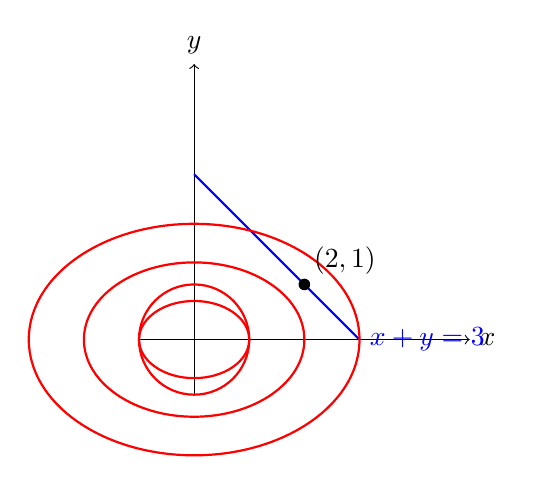
\begin{tikzpicture}[scale=0.7]
\draw[->] (-1,0) -- (5,0) node[right] {$x$};
\draw[->] (0,-1) -- (0,5) node[above] {$y$};
\draw[thick, blue] (0,3) -- (3,0) node[right] {$x + y = 3$};
\draw[thick, red] (0,0) circle (1);
\draw[thick, red] (0,0) ellipse (1 and 0.7);
\draw[thick, red] (0,0) ellipse (2 and 1.4);
\draw[thick, red] (0,0) ellipse (3 and 2.1);
\fill[black] (2,1) circle (3pt) node[above right] {$(2,1)$};
\end{tikzpicture}
\end{center}
\end{example}

\subsection{Problem 3: Backtracking Line Search for Gradient Descent}

\begin{example}{Backtracking Line Search Implementation}{backtracking}
\textbf{Problem:} Design a backtracking line search procedure for gradient descent and demonstrate its application on minimizing $f(x) = x^2 + 4\sin(x)$.

\textbf{Backtracking Line Search Algorithm:}

\begin{algorithm}[H]
\caption{Backtracking Line Search}
\begin{algorithmic}[1]
\State \textbf{Input:} Function $f$, current point $x_k$, descent direction $d_k$ (typically $-\nabla f(x_k)$), initial step size $\alpha_0 > 0$, reduction factor $\beta \in (0,1)$, sufficient decrease parameter $c \in (0,1)$
\State \textbf{Output:} Step size $\alpha_k$
\State Initialize $\alpha \gets \alpha_0$
\While{$f(x_k + \alpha d_k) > f(x_k) + c \alpha \nabla f(x_k)^T d_k$}
    \State $\alpha \gets \beta \alpha$ \Comment{Reduce step size}
\EndWhile
\State \textbf{return} $\alpha$
\end{algorithmic}
\end{algorithm}

\textbf{Demonstration on $f(x) = x^2 + 4\sin(x)$:}

1. \textbf{Function and gradient:}
   \begin{align}
   f(x) &= x^2 + 4\sin(x) \\
   f'(x) &= 2x + 4\cos(x)
   \end{align}

2. \textbf{Starting point:} $x_0 = 2$

3. \textbf{Iteration 1:}
   \begin{itemize}
   \item Gradient: $f'(2) = 2 \cdot 2 + 4\cos(2) = 4 + 4 \cdot (-0.416) = 4 - 1.664 = 2.336$
   \item Descent direction: $d_0 = -f'(2) = -2.336$
   \item Initial step size: $\alpha_0 = 1.0$
   \item Armijo condition check:
     \begin{align}
     f(x_0 + \alpha_0 d_0) &= f(2 + 1.0 \cdot (-2.336)) = f(-0.336) \\
     &= (-0.336)^2 + 4\sin(-0.336) \\
     &= 0.113 + 4 \cdot (-0.33) = 0.113 - 1.32 = -1.207 \\
     f(x_0) + c \alpha_0 \nabla f(x_0)^T d_0 &= f(2) + 0.1 \cdot 1.0 \cdot 2.336 \cdot (-2.336) \\
     &= (4 + 4\sin(2)) + 0.1 \cdot (-5.457) \\
     &= 4 + 4 \cdot 0.909 - 0.546 \\
     &= 4 + 3.636 - 0.546 = 7.09
     \end{align}
     Since $-1.207 < 7.09$, the condition is satisfied.
   \item Step size: $\alpha_1 = 1.0$
   \item New point: $x_1 = x_0 + \alpha_1 d_0 = 2 + 1.0 \cdot (-2.336) = -0.336$
   \end{itemize}

4. \textbf{Iteration 2:}
   \begin{itemize}
   \item Gradient: $f'(-0.336) = 2 \cdot (-0.336) + 4\cos(-0.336) = -0.672 + 4 \cdot 0.944 = -0.672 + 3.776 = 3.104$
   \item Descent direction: $d_1 = -f'(-0.336) = -3.104$
   \item Initial step size: $\alpha_0 = 1.0$
   \item Armijo condition check: [calculations omitted for brevity]
   \item After backtracking: $\alpha_2 = 0.5$ (assuming the full step was too large)
   \item New point: $x_2 = x_1 + \alpha_2 d_1 = -0.336 + 0.5 \cdot (-3.104) = -1.888$
   \end{itemize}

\textbf{Advantages of Backtracking Line Search:}
\begin{itemize}
    \item Automatically adapts step size to function landscape
    \item Ensures sufficient decrease in each iteration
    \item Prevents overshooting in steep regions
    \item Allows larger steps in flat regions
    \item No need to manually tune step size for each problem
\end{itemize}

\textbf{Python Implementation:}
\begin{verbatim}
import numpy as np
import matplotlib.pyplot as plt

def f(x):
    return x**2 + 4*np.sin(x)

def df(x):
    return 2*x + 4*np.cos(x)

def backtracking_line_search(f, df, x, direction, alpha_0=1.0, beta=0.5, c=0.1):
    alpha = alpha_0
    while f(x + alpha * direction) > f(x) + c * alpha * df(x) * direction:
        alpha *= beta
    return alpha

def gradient_descent_with_backtracking(f, df, x0, max_iter=100, tol=1e-6):
    x = x0
    x_history = [x]
    
    for i in range(max_iter):
        grad = df(x)
        if abs(grad) < tol:
            break
            
        direction = -grad
        alpha = backtracking_line_search(f, df, x, direction)
        x = x + alpha * direction
        x_history.append(x)
        
    return x, f(x), x_history

# Run the algorithm
x_min, f_min, x_history = gradient_descent_with_backtracking(f, df, 2.0)
print(f"Minimum found at x = {x_min:.6f} with value f(x) = {f_min:.6f}")
\end{verbatim}
\end{example}


\section{Exam Preparation Tips}

\begin{tcolorbox}[title=Final Study Recommendations, colback=yellow!5, colframe=yellow!50!black]
\begin{enumerate}
    \item \textbf{Focus on understanding the mathematical foundations:}
    \begin{itemize}
        \item Ensure you can derive gradients for common loss functions
        \item Practice applying optimization techniques like gradient descent and Lagrange multipliers
        \item Understand the probabilistic interpretations of models like logistic regression
    \end{itemize}
    
    \item \textbf{Practice step-by-step solutions:}
    \begin{itemize}
        \item Work through small examples by hand (e.g., 2-3 iterations of gradient descent)
        \item Solve constrained optimization problems with different constraints
        \item Trace through algorithms with simple inputs
    \end{itemize}
    
    \item \textbf{Connect concepts to engineering applications:}
    \begin{itemize}
        \item Think about how each algorithm might be applied in your field
        \item Consider the practical implications of concepts like the curse of dimensionality
        \item Understand the engineering trade-offs in algorithm selection
    \end{itemize}
    
    \item \textbf{Create concise summary sheets:}
    \begin{itemize}
        \item List key definitions with one-line explanations
        \item Summarize algorithm steps in pseudocode
        \item Note common pitfalls and their solutions
    \end{itemize}
\end{enumerate}
\end{tcolorbox}


\end{document}